\section{Durchführung}
\label{sec:Durchführung}
\begin{figure}
    \centering
    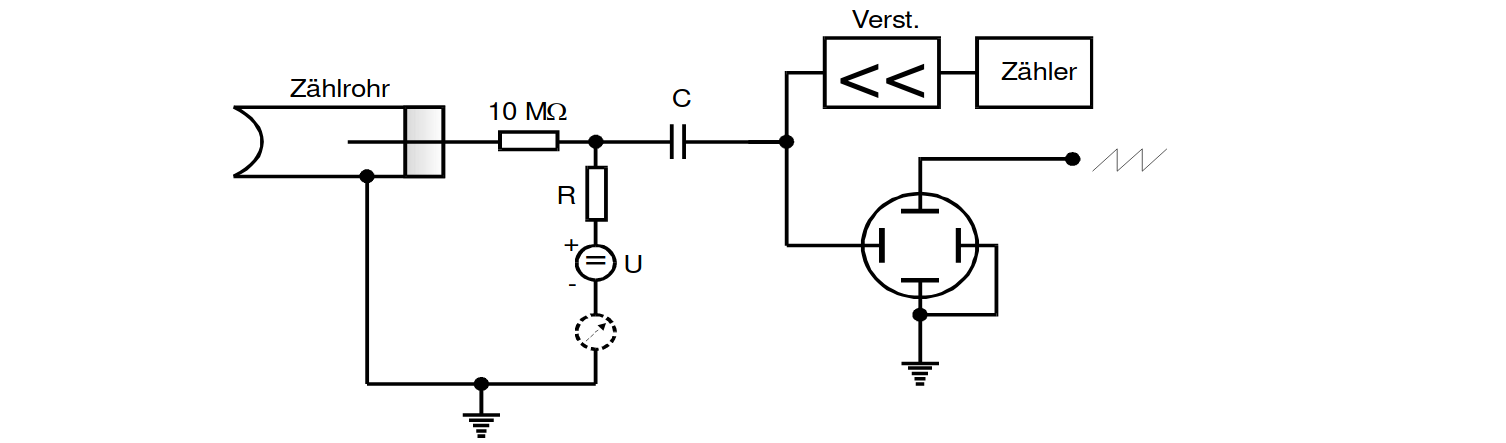
\includegraphics[width=\textwidth]{messapparatur.png}
    \caption{Skizze der Messapparatur \cite{7}{anleitung}}
    \label{fig:messapparatur}
\end{figure}
In der \autoref{fig:messapparatur} ist der Versuchsaufbau zu sehen.
Die in Zählrohr entstehende Ladung $Q$ läuft durch den Draht über den Widerstand $R$ ab.
Dort wird ein Spannungsimpuls erzeugt, der durch den Kondensator $C$ entkoppelt wird.
Anschließend wird der Impuls einmal verstärkt und dann im Zähler registriert, sowie auf dem Oszillographenschirm angezeigt.\\
\\
Vor dem Zählrohr wird eine $\ce{^{204}Tl}$ Quelle positioniert, so dass bei einer mittleren Zählrohrspannung die Zählrate unter  $\num{100}$ Imp/s bleibt.
Nun wird die Spannung in Schritten von $\increment U = \SI{10}{\volt}$ erhöht und dort jeweils mit einer Integrationszeit $t=\SI{60}{\second}$ die Zählrate notiert.\\
Dabei wird in Abständen von $\increment U = \SI{50}{\volt}$ der Zählrohrstrom $I$ am Amperemeter abgelesen.\\
\\
Zur Bestimmung der Totzeit am Oszilloskop wird die Zeitablenkung durch die Anstiegsflanke der Zählrohrimpulse getriggert, sodass sich ein Bild wie in \autoref{fig:totzeit} dargestellt wird.
Bei bekannter Ablenkgeschwindigkeit des Kathodenstrahls ist die Totzeit abzulesen. \\
Für die Bestimmung der Totzeit mit der Zwei-Quellen-Methode wird bei einer Messzeit von $t=\SI{120}{\second}$ die zuerst die Zählrate $N_1$ der $\ce{^{204}Tl}$-Quelle gemessen.
Ohne die Position der ersten Quelle zum Zählrohr zu verändern, wird eine zweite hinzugefügt und die Zählrate $N_{1+2}$ aufgeschrieben.
Anschließend wird die erste Quelle entfernt und die Zählrate $N_2$ der zweiten Quelle gemessen.